\documentclass{article}
\title{Calibrazione di una termocoppia}
\author{Lorenzo Redighieri\\Luca Zoppetti}
\date{16 Novembre 2022}

\usepackage[margin=100pt]{geometry}

\usepackage{graphicx}
\graphicspath{ {./images/} }

\usepackage{float}

\usepackage{wrapfig}

\usepackage{gensymb}

\usepackage{amssymb}

\usepackage{amsmath}

\usepackage{xfrac}

\usepackage{cite}

\renewcommand{\contentsname}{Contenuti}

\renewcommand{\abstractname}{Abstract}

\renewcommand{\refname}{Bibliografia}

\renewcommand{\figurename}{Figura}

\begin{document}

\maketitle

\begin{abstract}
L'oggetto dell'analisi sperimentale è stata una termocoppia, ossia uno strumento che sfrutta l'effetto Seebeck per misurare la temperatura di un corpo. L’obiettivo dell’esperienza è stato studiare la correlazione fra la temperatura misurata a un'estremità dell'apparato e la differenza di potenziale registrata fra i due giunti dello stesso. A tal fine sono stati raccolti dei dati che sono poi stati analizzati con l’ausilio di Excel e del framework ROOT. I risultati suggeriscono una dipendenza lineare fra la temperatura e la differenza di potenziale. Inoltre, vengono presentate due ulteriori analisi in merito alla temperatura del giunto freddo e alla dipendenza della temperatura dal tempo in fase di raffreddamento del sistema.
\end{abstract}

\newpage

\section{Introduzione}
La termocoppia è uno strumento composto da due giunzioni bimetalliche che, quando mantenute a temperature diverse, generano una differenza di potenziale dell’ordine di $10^{-3}V$ dovuta al diverso comportamento degli elettroni nei due metalli. Questo meccanismo è comunemente chiamato “effetto Seebeck” \cite{seebeck}. Per sfruttarlo, una delle due giunzioni, il “giunto freddo”, è mantenuta a temperatura costante e collegata al voltmetro, mentre l’altra, il “giunto caldo”, è inserita nel sistema in misura.

La prima grandezza presa in esame nel corso dell’esperienza è stata la differenza di potenziale registrata dalla termocoppia, misurata in $mV$ e indicata come $V$. L’altra è stata la temperatura di riferimento indicata da un termistore posto nel sistema in misura, misurata in $\degree C$ e indicata come $T$.

Queste due grandezze sono state innanzitutto utilizzate per calcolare i parametri $A \medspace (mV)$ e $B \medspace (mV/\degree C)$ della retta di calibrazione, confrontando il valore di $B$ con quello accettato $B_0 \approx 40 \mu V/\degree C$. In un secondo momento, è stata calcolata la temperatura del giunto freddo della termocoppia. Infine, con i dati raccolti durante la fase di raffreddamento, si è calcolato il parametro $k$ di raffreddamento che compare nella legge di Newton sulla dipendenza della temperatura dal tempo.

\section{Metodo sperimentale}
\subsection{Apparato sperimentale}
Per questo esperimento si è deciso di utilizzare una termocoppia di tipo K (chromel-alumel) con risoluzione $0,03mV$ e un termistore, un particolare termometro il cui funzionamento si basa sulla dipendenza della resistività elettrica dalla temperatura. Ai fini della regressione lineare l'incertezza sulle temperature, essendo trascurabile, è stata considerata nulla durante l'intero esperimento. I sensori sono stati collegati a una scheda di presa dati NI ELVIS II (Fig. \ref{apparato_sperimentale}), la quale trasmette i dati al computer, che poi li rappresenta attraverso un programma scritto in LabVIEW\footnote{Per maggiori dettagli in merito al programma in LabVIEW si rimanda alla sezione \textbf{\ref{acquisizione_dati}}.}. Oltre alla strumentazione scientifica sono stati utilizzati un becher, un tritaghiaccio e una resistenza per scaldare il sistema (Fig. \ref{becher_trita}).

\begin{figure}[h!] %foto dell'apparato sperimentale
\centering
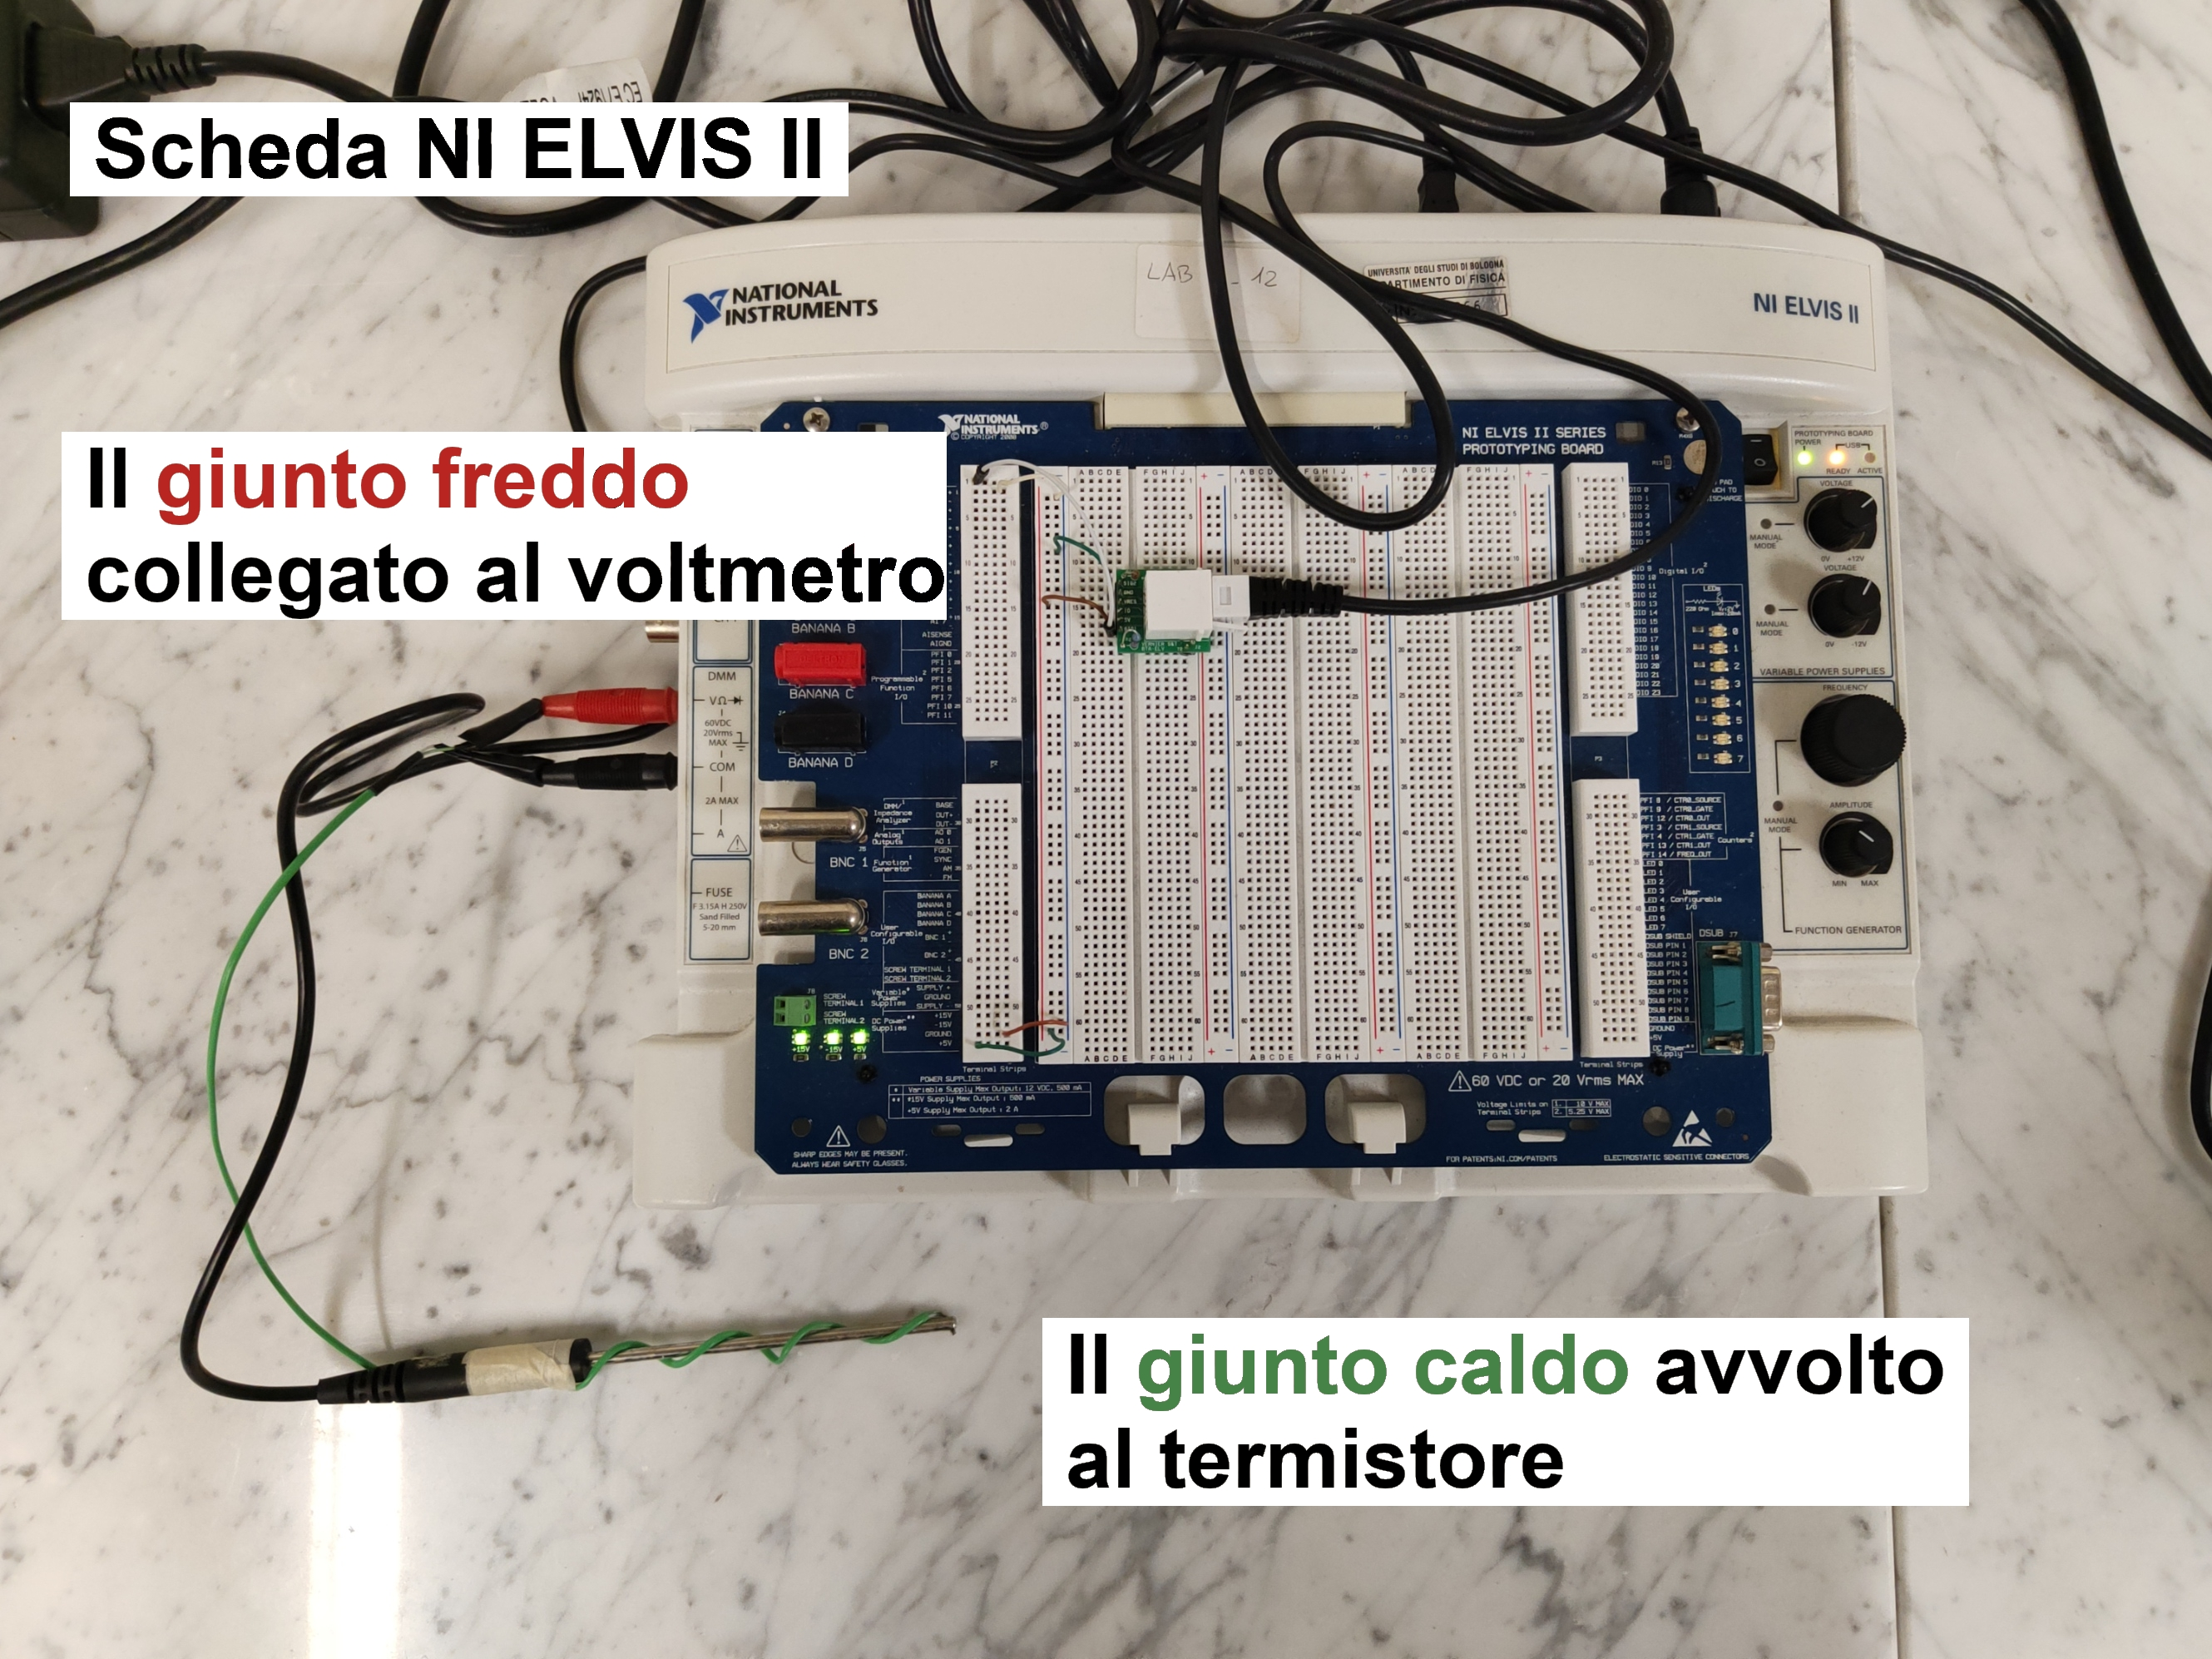
\includegraphics[width=0.49\textwidth]{elvis}
\caption{La scheda NI ELVIS II collegata alla termocoppia, il cui giunto caldo si trova all'estremità del cavo verde, e al termistore, collegato al cavo nero.}
\label{apparato_sperimentale}
\end{figure}

\begin{figure}[h!]
\centering
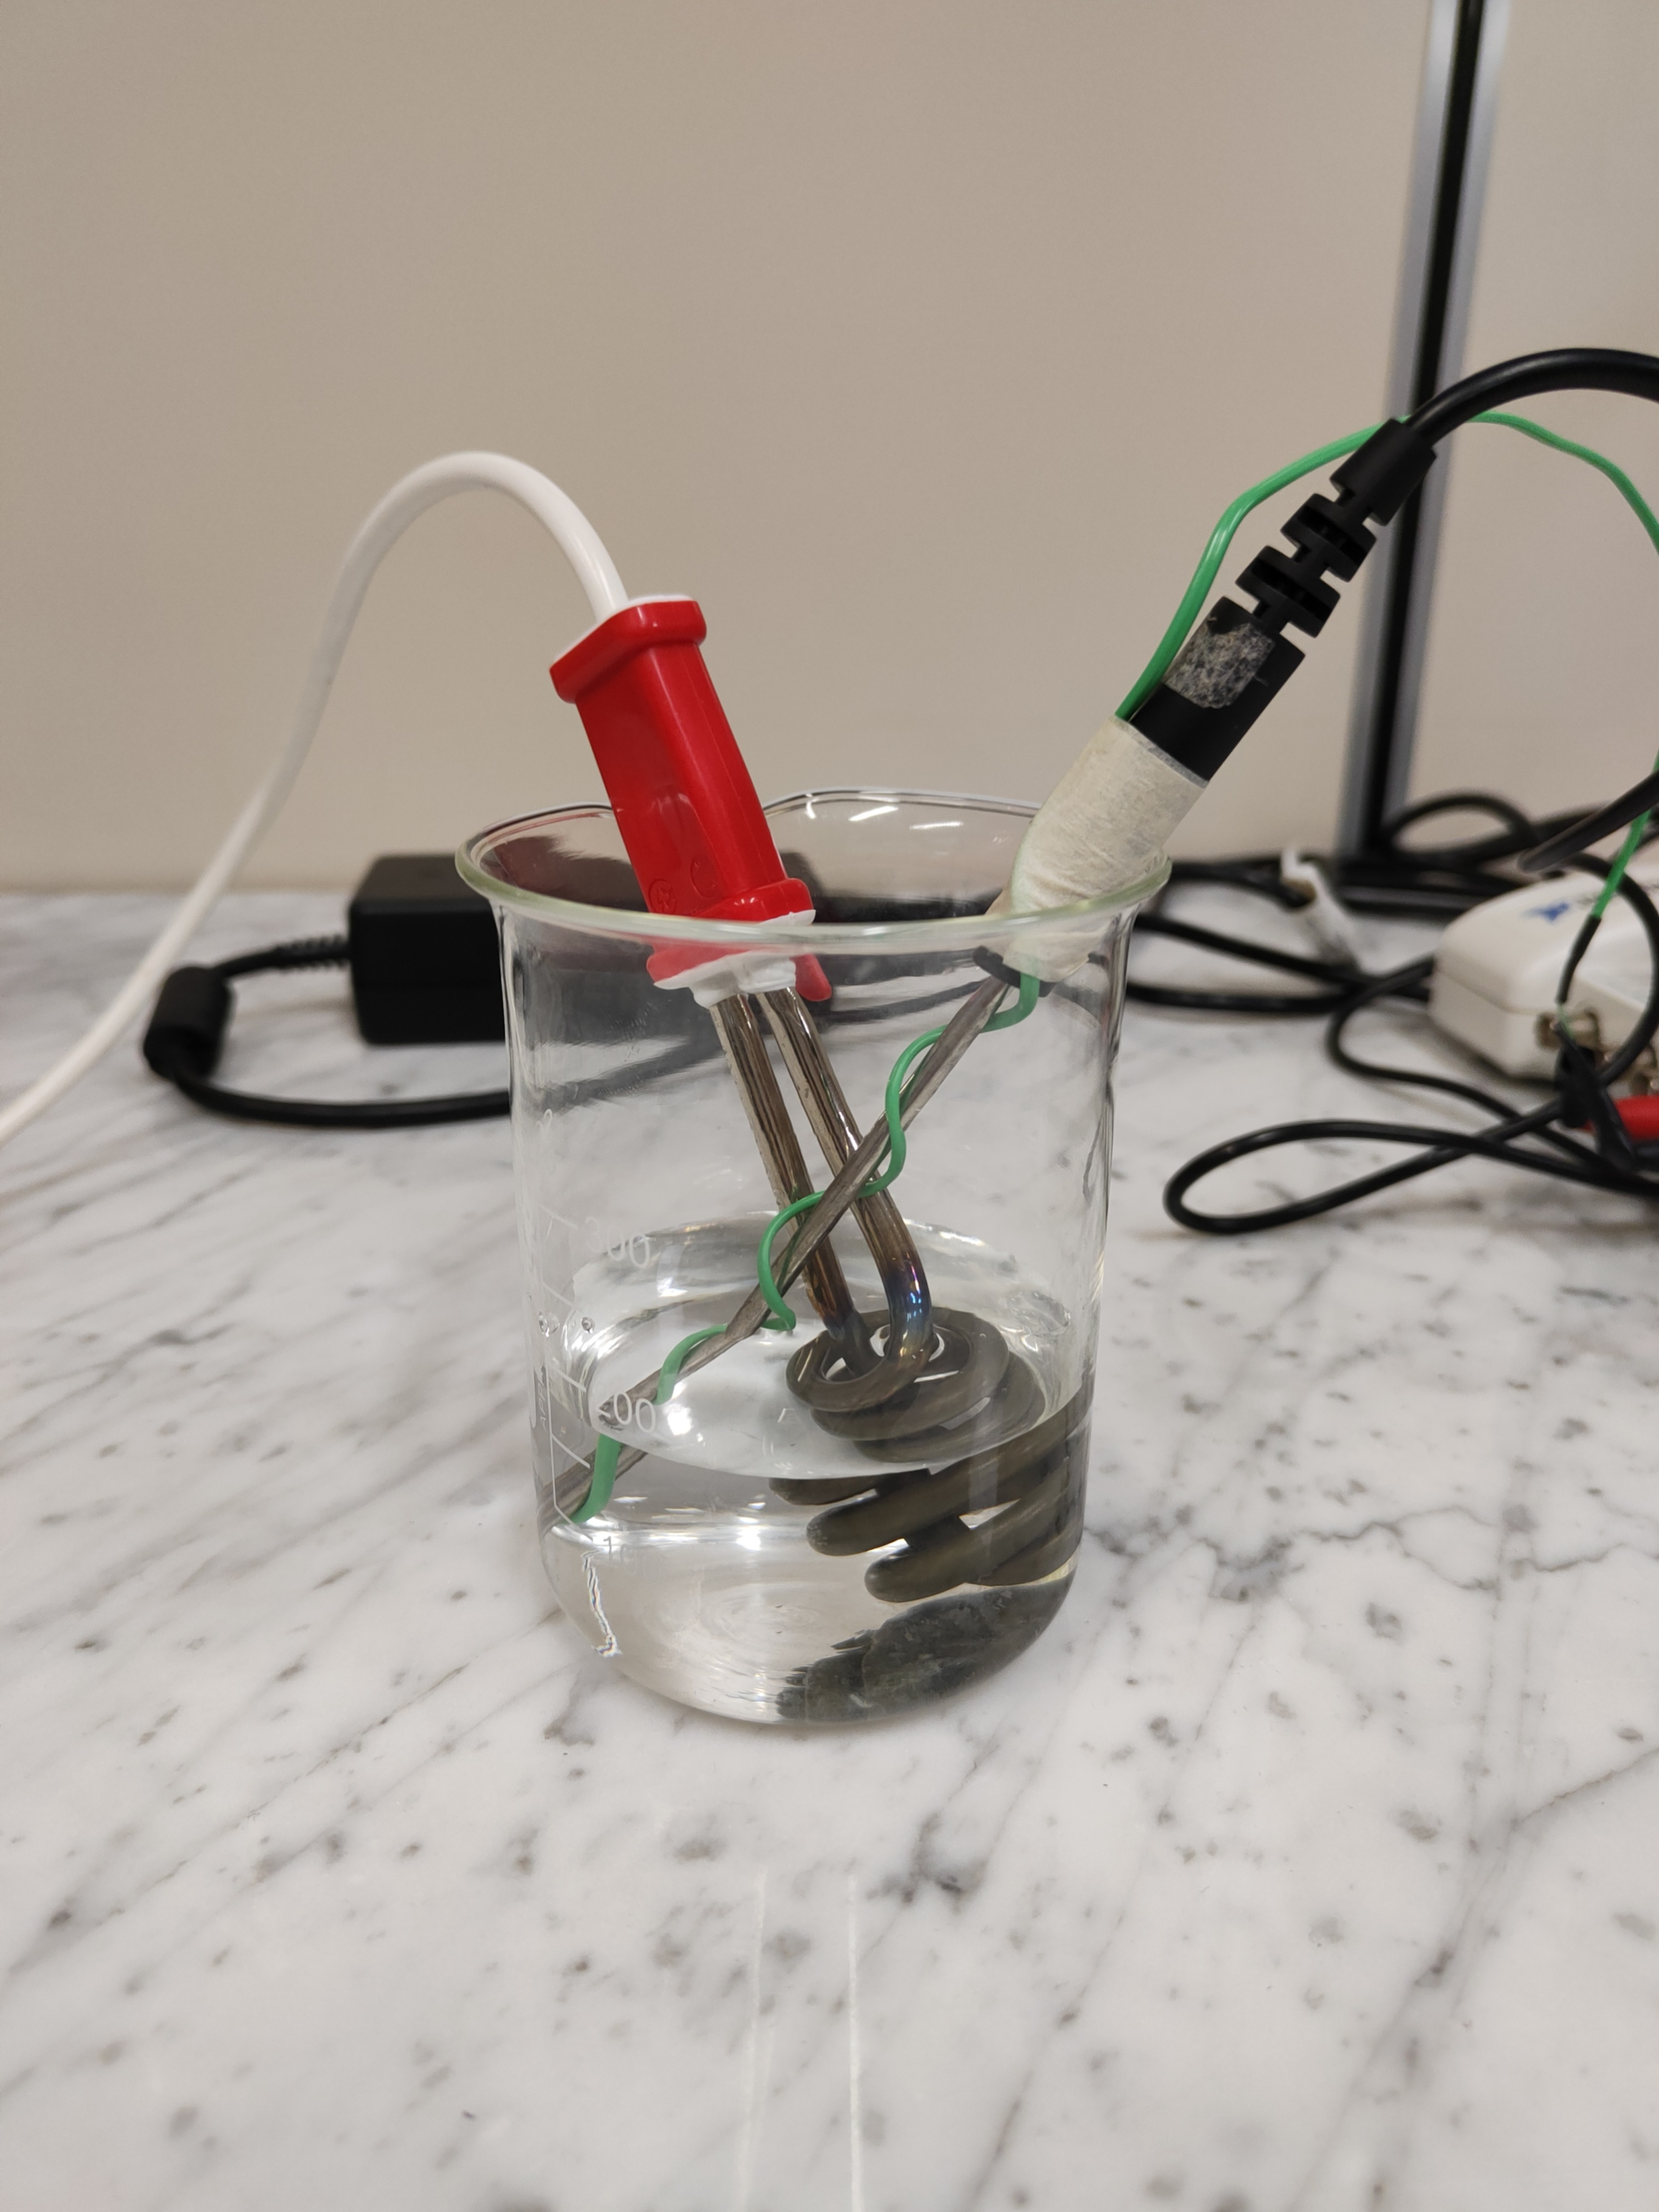
\includegraphics[width=0.27\textwidth]{becher}
\hspace{60pt}
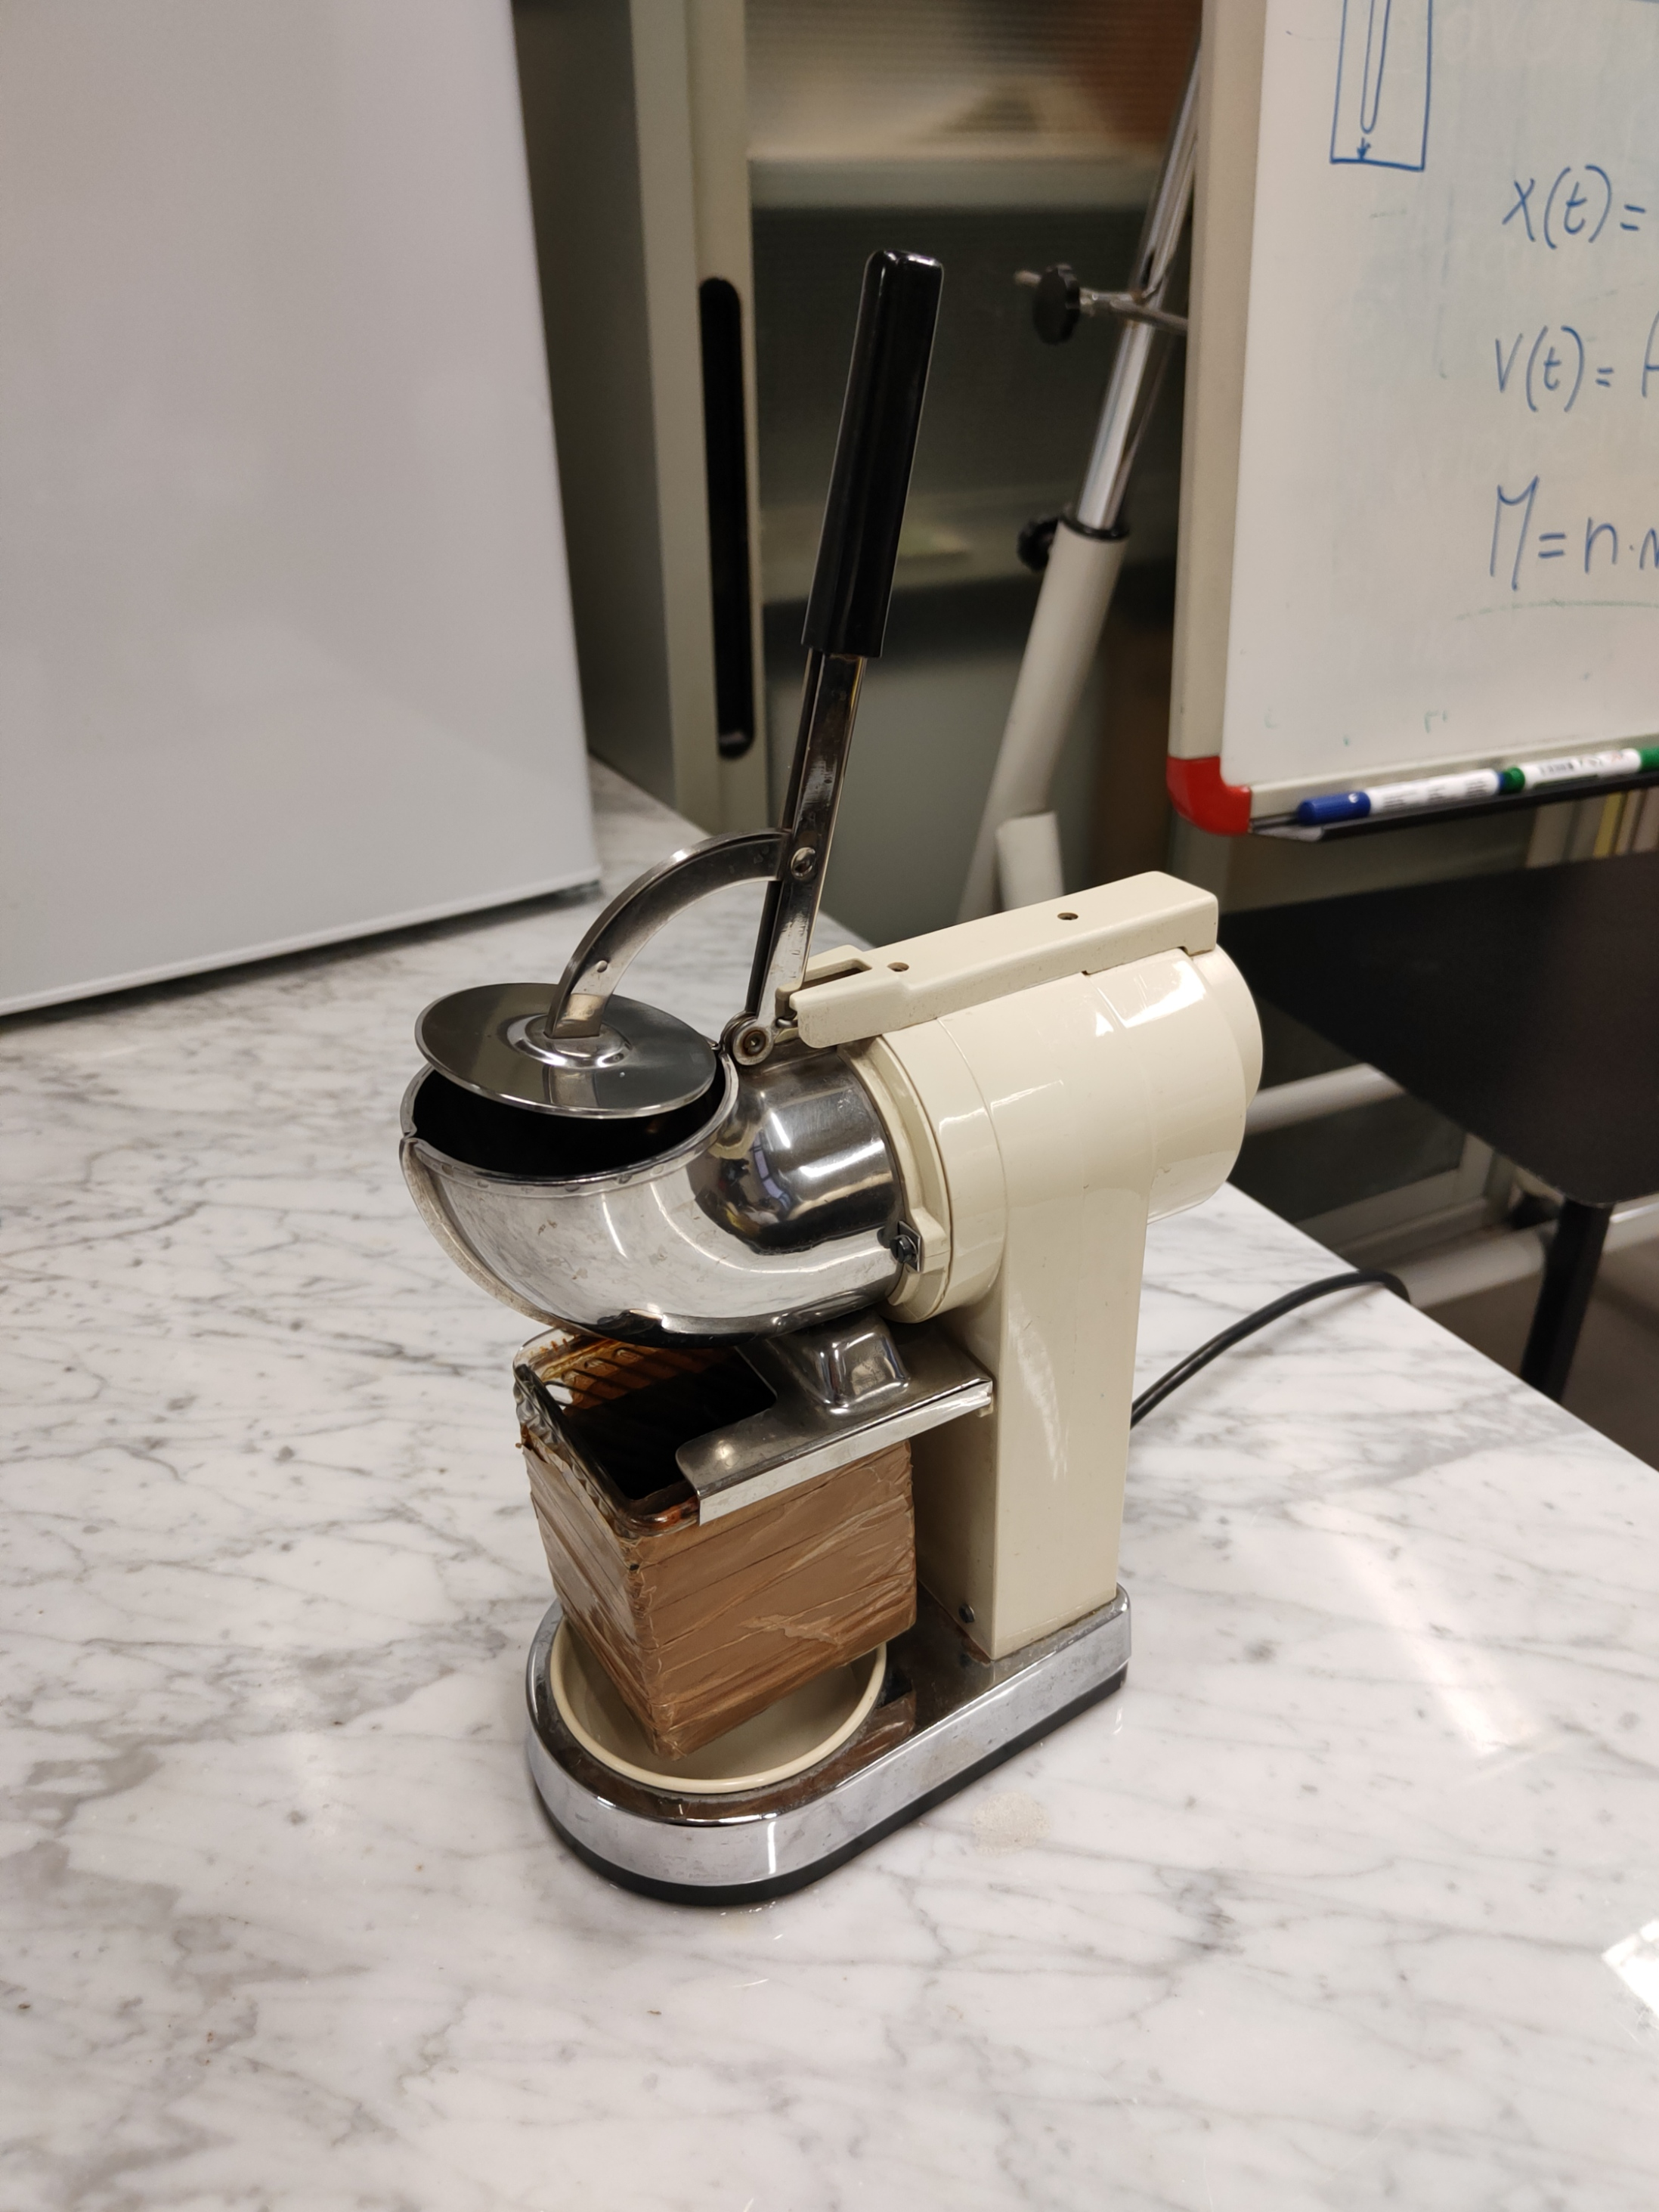
\includegraphics[width=0.27\textwidth]{ice}
\caption{A sinistra, la resistenza e il giunto caldo della termocoppia avvolto al termistore inseriti nel becher. A destra, il tritaghiaccio utilizzato.}
\label{becher_trita}
\end{figure}

\subsection{Svolgimento}
Dopo aver preparato l’apparato sperimentale, è stato utilizzato un tritaghiaccio per ridurre in piccoli pezzi una decina di blocchetti di ghiaccio estratti dal freezer. Per velocizzare lo scioglimento è stata aggiunta dell'acqua distillata che, una volta arrivata a temperatura ambiente ($ T_{amb} \approx 22 \degree C $), è stata scaldata dalla resistenza precedentemente mostrata. Nella fase di riscaldamento sono stati registrati dati a intervalli di circa $10\degree C$ con il programma in LabVIEW. Raggiunta la temperatura di ebollizione ($T_e \approx 100 \degree C$), la resistenza è stata rimossa dal becher per iniziare a registrare i dati della fase di raffreddamento. Nei successivi 30 minuti, tramite il programma in LabVIEW sono stati raccolti dati a intervalli di circa $10\degree C$, mentre in una tabella Excel sono state annotate le temperature a intervalli di un minuto. 

Con le formule della regressione lineare\footnote{Per le formule della regressione lineare si rimanda all'appendice.} \cite{taylor} sono stati calcolati, sia in fase di salita che di discesa, i parametri $A$ e $B$ della retta di calibrazione della termocoppia, che è nella forma $V(T)=A+BT$.

Sapendo che se le due giunzioni della termocoppia si trovano alla stessa temperatura non si genera alcuna differenza di potenziale, si è calcolata la temperatura del giunto freddo $T_f$ attraverso la seguente relazione:

$$V(T_f)=A+BT_f=0$$
$$T_f=-\frac{A}{B}$$

È riportata di seguito la formula della legge di raffreddamento di Newton, dove $T_{amb}$ indica la temperatura ambiente, $T_{iniz}$ la temperatura iniziale del sistema, $e \approx 2.718$ il numero di Eulero e $k$ il parametro che rappresenta la rapidità con la quale il liquido si raffredda\footnote{Più precisamente, l’inverso del parametro $k$ rappresenta il tempo necessario affinchè il rapporto $\frac{T-T_{amb}}{T_{iniz}-T_{amb}}$ si riduca di un fattore pari a $e$.}.

$$
T(t)-T_{amb}=(T_{iniz}-T_{amb})e^{-kt}
$$

Utilizzando un foglio di calcolo, è stato determinato il parametro $k$ ed è stata verificata la corrispondenza fra la legge sopra riportata e i dati raccolti nella fase di discesa.

\section{Risultati}

\subsection{Acquisizione dati}
\label{acquisizione_dati}
Per gestire i dati dell'esperimento è stato utilizzato un programma scritto in LabVIEW dotato di un'interfaccia grafica in grado di rappresentare le misurazioni in un piano cartesiano. Lungo l'asse delle ascisse veniva mostrata la temperatura in gradi celsius, mentre in quello delle ordinate la differenza di potenziale in millivolt.
Per permettere al computer di ricevere le informazioni derivanti dalle misurazioni è stata impiegata una scheda ELVIS, alla quale sono stati collegati il termistore e la termocoppia, rispettivamente all'ingresso $V/\Omega$ del multimetro e ad un canale. In seguito, a partire dai dati raccolti, è stata effettuata una regressione lineare, col fine di determinare la costante che lega $V$ e $T$. Le misure e la retta di calibrazione risultante sono riportate nella Fig. \ref{grafici_termocoppia}.

\begin{figure}[h!] %grafici (termocoppia)
\centering
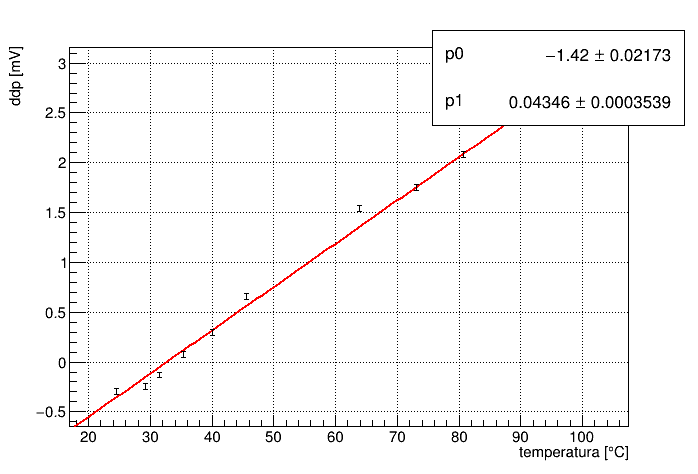
\includegraphics[width=0.45\textwidth]{tc_salita_root}
\hspace{20pt}
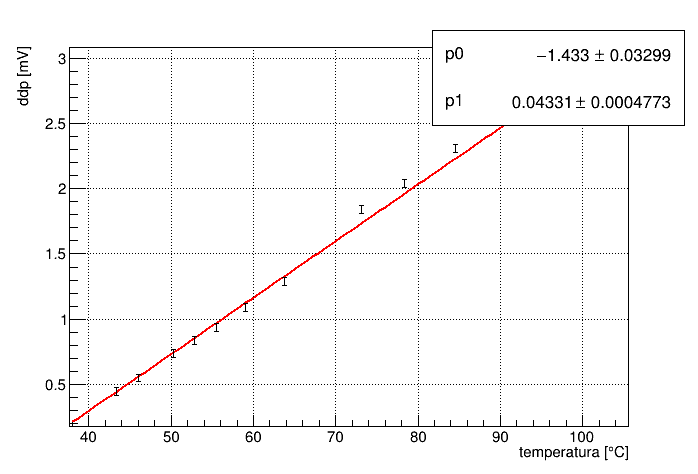
\includegraphics[width=0.45\textwidth]{tc_discesa_root}
\caption{Andamento della temperatura ($\degree C$) del giunto caldo in funzione della differenza di potenziale ($mV$) generata nella termocoppia. Il grafico a sinistra mostra l'andamento durante la fase di riscaldamento, quello a destra durante la fase di raffreddamento. Entrambi i grafici sono stati costruiti col programma di analisi in ROOT.}
\label{grafici_termocoppia}
\end{figure}

Durante la fase di raffreddamento, è stata monitorata la variazione della temperatura in funzione del tempo. In particolare, ogni minuto è stata misurata la temperatura dell'acqua, per un totale di trenta misure. Successivamente, sono stati considerati tre intervalli di tempo da 10 minuti ciascuno e per ognuno di essi è stato calcolato il parametro $k$ che regola la legge di raffreddamento di Newton (Fig. \ref{grafici_newton}).


\begin{figure}[h!] %grafici (raffreddamento Newton)
\centering
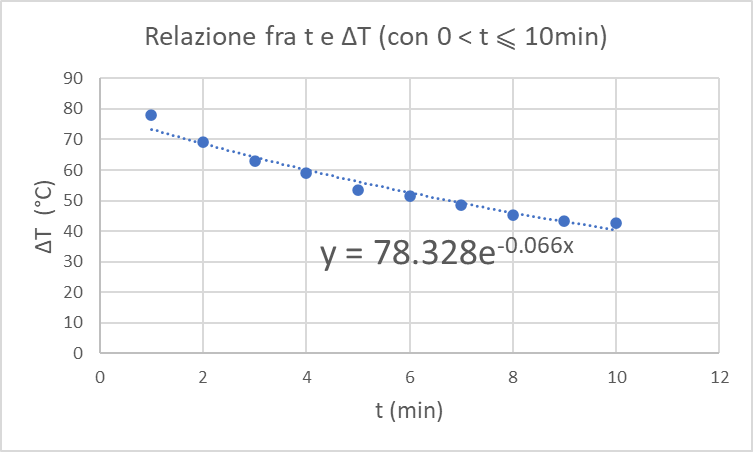
\includegraphics[width=0.3\textwidth]{n1}
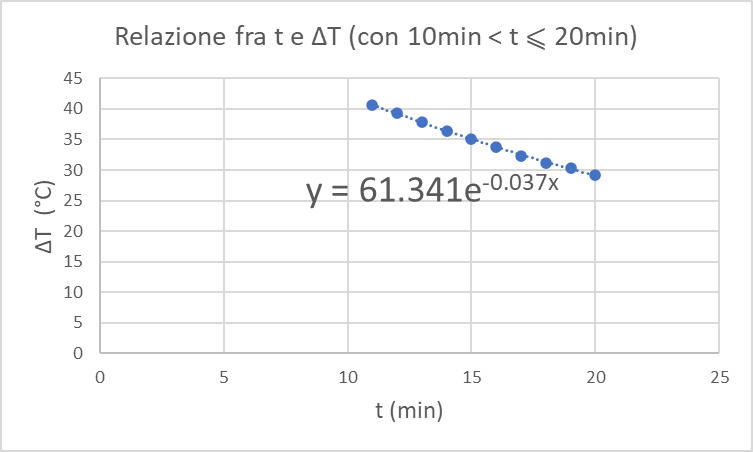
\includegraphics[width=0.3\textwidth]{n2}
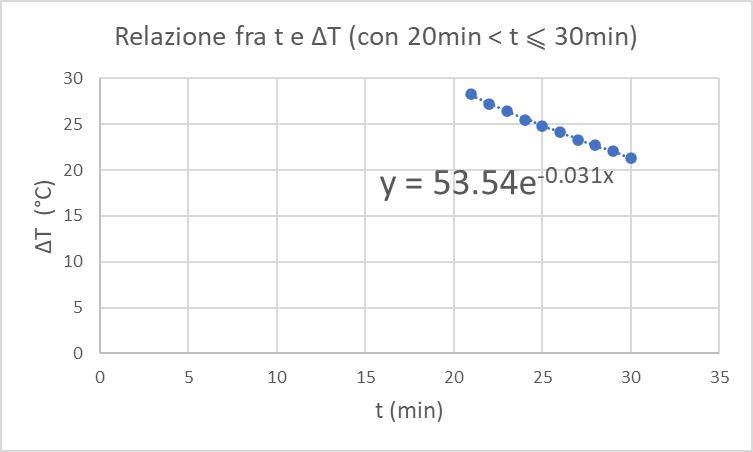
\includegraphics[width=0.3\textwidth]{n3}
\caption{Andamento esponenziale della temperatura in funzione del tempo durante la fase di raffreddamento. Sono state effettuate 30 misure in 30 minuti (una ogni minuto). Da sinistra a destra, i grafici si riferiscono agli intervalli di tempo: $0 < t \leqslant 10min$, $10min < t \leqslant 20min$, $20min < t \leqslant 30min$. I tre grafici sono stati realizzati con Excel.}
\label{grafici_newton}
\end{figure}

\subsection{Elaborazione dati e risultati quantitativi}
\subsubsection{Termocoppia}
Le coppie $(T,V)$ sono state divise in due gruppi: uno contenente i dati relativi alla fase di riscaldamento, l'altro a quella di raffreddamento. A partire da tali dati, sono state effettuate due regressioni lineari (una per ogni gruppo),  che hanno prodotto i risultati riportati nella tabella seguente:

\begin{center}
\begin{tabular}{|c|c|c|}
\hline
 & Riscaldamento & Raffreddamento \\
\hline
$ A \medspace (mV) $ & $ -1.42 \pm 0.02 $ & $ -1.43 \pm 0.03 $ \\
\hline
$ B \medspace (mV/\degree C) $ & $ 0.0435 \pm 0.0004 $ & $ 0.0433 \pm 0.0005 $ \\
\hline
\end{tabular}
\end{center}

\noindent Dalla Fig. \ref{grafici_termocoppia} si può notare chiaramente che alcune misure non sono compatibili con la retta di calibrazione. Da ciò si deduce che tali discrepanze non possono essere ricondotte a fluttuazioni puramente statistiche, bensì sono il risultato di errori sistematici.

\subsubsection{Giunto freddo}
Grazie ai parametri della retta di calibrazione della termocoppia è possibile calcolare la temperatura del giunto freddo ($T_f$). Essa è stata calcolata sia utilizzando i parametri della fase di riscaldamento, sia quelli della fase di raffreddamento, dando i seguenti risultati:

\begin{center}
\begin{tabular}{|c|c|c|}
\hline
 & Riscaldamento & Raffreddamento \\
\hline
$ T_f \medspace (\degree C) $ & $ 32.7 \pm 0.8 $ & $ 33.1 \pm 1.1 $ \\
\hline
\end{tabular}
\end{center}

\noindent Le due misure sono compatibili tra loro. Inoltre, è plausibile che la temperatura del giunto freddo risulti più elevata rispetto alla temperatura ambiente del laboratorio ($ T_{amb} \approx 22 \degree C $) a causa della scheda ELVIS. La scheda, essendo formata da componenti elettronici, si è surriscaldata durante l'acquisizione dei dati per via dell'effetto Joule \cite{joule}, trasferendo calore agli oggetti vicini (tra cui il giunto freddo).

\subsubsection{Legge di raffreddamento di Newton}
Le trenta misure della temperatura prese durante la fase di raffreddamento sono state divise in tre gruppi, il primo contenente le misure raccolte nei primi dieci minuti, il secondo quelle raccolte nei dieci minuti seguenti e il terzo quelle raccolte negli ultimi dieci minuti. Con l'aiuto di un foglio di calcolo, è stato ricavato il parametro $k$ relativo a ciascun gruppo, producendo i seguenti risultati:

\begin{center}
\begin{tabular}{|c|c|c|c|}
\hline
 & $ 0 < t \leqslant 10min $ & $ 10min < t \leqslant 20min $ & $ 20min < t \leqslant 30min $ \\
\hline
$ k \medspace (min^{-1}) $ & 0.066 & 0.037 & 0.031 \\
\hline
\end{tabular}
\end{center}

\noindent Il motivo di una differenza così ampia fra i tre valori del parametro $k$ potrebbe risiedere in alcuni effetti non trascurabili (come lo scambio di calore per evaporazione dell’acqua e il raffreddamento attraverso le pareti del becher) che portano ad una diminuzione della temperatura nel tempo non esattamente rappresentabile come un’unica esponenziale. \\
Calcolando la media di questi tre valori è possibile stimare $k$, a cui è associata un'incertezza pari alla semidispersione massima\footnote{Per la formula della semidispersione massima si rimanda all'appendice.} del campione:
$$ k = ( 0.045 \pm 0.018 ) min ^ {-1} $$


\section{Conclusioni}
Le misure indirette di $A$ e di $B$ durante le fasi di riscaldamento e raffreddamento sono compatibili tra di loro, ma nessuna delle due restituisce un parametro $B$ e un'incertezza $\sigma_B$ compatibili con il valore accettato $B_0 \approx 40 \mu V/\degree C$. Se ne deduce che i risultati sono stati alterati da errori sistematici occorsi durante l'esecuzione dell'esperimento.

Anche le due misure indirette della temperatura del giunto freddo risultano compatibili tra loro. Teoricamente tale temperatura dovrebbe essere uguale alla temperatura ambiente, tuttavia, come già spiegato in precedenza, è normale che essa sia maggiore di quella del laboratorio a causa dell'apparato sperimentale.

La rappresentazione grafica delle temperature in funzione del tempo registrate in fase di raffreddamento rispetta l'andamento esponenziale previsto dalla legge di raffreddamento di Newton. Ciononostante, i valori discordanti del parametro $k$ fanno pensare alla presenza di effetti non trascurabili dovuti alla conformazione del sistema in misura.

\newpage

\begin{thebibliography}{9}
\bibitem{seebeck}
Encyclopedia Britannica, “Seebeck effect”; Britannica, The Editors of Encyclopaedia (1998) https://www.britannica.com/science/Seebeck-effect.

\bibitem{taylor}
J. R. Taylor, “Introduzione all'analisi degli errori”; Zanichelli (2000) pag. 185.

\bibitem{joule}
Encyclopedia Britannica, “Joule heating”; Britannica, The Editors of Encyclopaedia (2022) https://www.britannica.com/science/Joules-law. 
\end{thebibliography}

\section*{Appendice}
\paragraph{Regressione lineare} Sapendo che due grandezze $x$ e $y$ sono legate da una relazione lineare ($ y = A + B x $), disponendo di $N$ misurazioni compiute su $x$ e $y$ e nelle ipotesi che le incertezze su $x$ siano trascurabili, che quelle su $y$ siano tutte uguali tra loro e che ogni $y_i$ sia estratto da una popolazione gaussiana,  è possibile stimare i parametri $A$ e $B$ con le rispettive incertezze $\sigma_A$ e $\sigma_B$ attraverso le seguenti formule:
$$ A = \dfrac{\displaystyle\sum_{i=1}^{N} x_i ^ 2 \displaystyle\sum_{i=1}^{N} y_i - \displaystyle\sum_{i=1}^{N} x_i \displaystyle\sum_{i=1}^{N} x_i y_i}{\Delta} \qquad
B = \dfrac{\displaystyle\sum_{i=1}^{N} x_i ^ 2 \displaystyle\sum_{i=1}^{N} y_i - \displaystyle\sum_{i=1}^{N} x_i \displaystyle\sum_{i=1}^{N} x_i y_i}{\Delta} $$
$$\sigma_A = \sigma_y \sqrt{\dfrac{\displaystyle\sum_{i=1}^{N} x_i ^ 2}{\Delta}} \qquad
\sigma_B = \sigma_y \sqrt{\dfrac{N}{\Delta}} \qquad
\text{con} \quad \Delta = N \displaystyle\sum_{i=1}^{N}x_i ^ 2 - \Bigg( \displaystyle\sum_{i=1}^{N}x_i \Bigg) ^ 2 $$

\paragraph{Semidispersione massima} Si definisce \textit{semidispersione massima} la metà della differenza fra il valore massimo di un campione e il valore minimo dello stesso. Essa rappresenta generalmente un modo poco affidabile di calcolare l'incertezza, ma ne restituisce una buona stima in caso di campioni molto ridotti.

$$ \sigma = \frac{x_{max}-x_{min}}{2} $$

\end{document}
